\chapter*{PREFACE}
\section*{ENGLISH}
Tens of millions of Americans, from Generation X-ers to baby boomers and beyond, are rediscovering Libertarianism, a visionary alternative to the
tired party orthodoxies of left and right. In 1995 a Gallup poll found that 52 percent of Americans said ``the federal government has become so large and powerful that it poses an immediate threat to the rights and freedoms of ordinary citizens.'' Later that year, \textit{The Wall Street Journal} concurred, saying: ``Because of their growing disdain for government, more and more Americans appear to be drifting--often unwittingly--toward a libertarian philosophy.''

Libertarianism is hardly new, but its framework for liberty under law and economic progress makes it especially suited for the dynamic new era we are now entering. In the United States, the bureaucratic leviathan is newly threatened by a resurgence of the libertarian ideas upon which the country was founded. We are witnessing a breakdown of all the cherished beliefs of the welfare-warfare state. Americans have seen the failure of big government. Now, in the 1990s, we are ready to apply the lessons of this century to make the next one the century not of the state but of the free individual.
\begin{figure}[!htb]
	\centering
	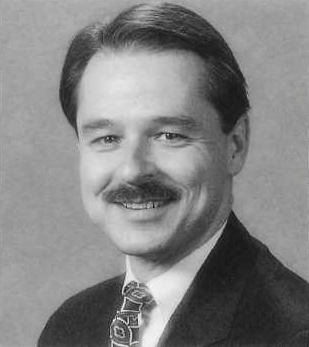
\includegraphics[width=0.7\textwidth]{0}
\end{figure}
David Boaz presents the essential guidebook to the libertarian perspective, detailing its roots, central tenets, solutions to contemporary policy dilemmas, and future in American politics. He confronts head-on the tough questions frequently posed to libertarians: What about inequality? Who protects the environment? What ties people together if they are essentially self-interested? A concluding section, ``Are You a Libertarian?'' gives readers a chance to explore the substance of their own beliefs. \textit{Libertarianism} is must reading for understanding one of the most exciting and hopeful movements of our time.

DAVID BOAZ is Executive Vice President of the Cato Institute, described by Rolling Stone as ``the hottest think-tank in Washington.'' His articles have appeared in \textit{The New York Times}, \textit{The Wall Street Journal}, \textit{The Washington Post}, and \textit{the Los Angeles Times}. He lives in Washington, D.C.
\newpage

\section*{中文版}
《古典自由主义:入门读物》在中国的出版象征着两个激动人心的进程:一是世界人民相互之间的距离变得越来越近;二是在经过一个世纪的战争与国家主义的肆虐之后,和平与自由的理念正在全世界范围内传播开来。

也许看上去这本书在中国的出版时机并不凑巧。目前,从法国总统到诺贝尔经济学奖得主都在宣称『自由放任资本主义完了』。一个美国中左派知识分子甚至欣喜若狂地说:『古典自由主义完蛋了』。这些批评家们是短视的。我们现在比以往任何时候都需要古典自由主义的理念---法治下的自由。

对于始于2008年末的这场经济危机,我们首要的任务是了解它,搞清楚它的起因。这是一次由政府管制、政府补贴和政府干预引起的危机,自然不可能用更多的管制、补贴和干预来治愈。克利斯托夫$\cdot$ 希钦斯在他的文章中说:『次贷与衍生金融工具的恐慌摧毁了我们对信用的信念,但是从某种意义上可以说,其起因是每个人都被许诺可以得到一切,而结果是每个人都上了民粹主义的当』。

在全世界范围内,美国经济常常被看作是自由放任资本主义的典范,的确,相对的开放、自由和较少的管制使得美国成了技术革命、经济增长和繁荣的火车头,但我们陷入这场经济危机正是因为悖离了自由放任资本主义的原则。美联储运用其权力压低利率,制造出廉价货币,从而鼓励人们购买房屋,造成房地产泡沫,而且联邦政府迫使银行和抵押公司把钱贷给不符合资格的贷款者。

『每个人都被许诺可以得到一切』---廉价货币,很容易获得的贷款,房地产价格的上涨。当所有的账单都同时到期的时候,联邦政府并不是让企业倒闭,而是插手让所有这些企业继续运转。这是国家资本主义的经济政策,不是古典自由主义政府的政策。

如果这场危机让我们开始质疑『美国式的资本主义』,这很好。如果说『美国式的资本主义』指的是中央货币当局操纵货币和信贷,中央政府每年征收3万亿美元税收并进行再分配,巨大的政府资助企业创造出由纳税人买单的双重垄断信贷市场,税法鼓励过度使用债务融资,以及政府迫使银行放出不良贷款的话,那么,反思这种『美国式的资本主义』也许是一件好事。

古典自由主义主张的是自由与责任,自由市场与公民自由,以及不踏入企血会议室和人们卧室的最小政府。很显然,古典自由主义从来就没有被列入克林顿和布什政府的议事日程。

尽管关于经济危机的原因有各种错误的解读,但是资本主义与古典自由主义的理念仍然充满活力。这个事实是不以那些批评家的意志为转移的。曾几何时,半个地球都拒绝资本主义。『自由世界』的著名知识分子都在担忧,中央计划经济显然将会在与资本主义国家的竞争中获胜,而某种资本主义与社会主义结合的模式将会是未来的潮流。但是,回头看看两种制度所导致的结果时,情况一目了然。无论是对比东德与西德,朝鲜与韩国,还是苏联与美国,人们很明显可以识别出那种笨拙、落后的制度。最好的结果是社会食滞不前,而最坏的结果则是独裁暴政。

与此同时,西方的那些半计划经济国家—--英国、新西兰、美国等—--也出现了经济僅化症,只不过表现得稍温和一些而已。从1970年代开始,很多这些国家都开始了消除价格管制,取消对市场竞争的限制,开放经济,削减税率与取消贸易壁垒的改革。铁幕两边的国家获得了广泛共识,那就是,私有财产和市场在组织现代经济运转中的作用是不可替代的。几乎与此同时发生的一场文化革命则让社会更加开放。在整个西方世界,妇女、少数民族、同性恋群体进入了社会主流。艺术、文学和生活方式变得更加多样化和个性化。60后一代与80后一代一起,让今天的美国进入了布林$\cdot$ 林赛在《丰裕时代》(The Age of Abundance)当中所说的『不知不觉的古典自由主义合流』时代。

有人认为,未来的时代政府会更强有力,另一些人則认为未来会是更广泛自由的时代。《理由》(\textit{Reason})杂志主编尼克$\cdot$格列斯派和马特$\cdot$ 韦尔奇写道:『我们事实上正生活在一个关键的时间点,这个时间点应当被称作古典自由主义时点。这是一个新时代的黎明。在这个新时代中,我们生活的每一个领域都高度个人化、个人选择的范围极大扩展$\cdots \cdots$ 事实上,现在的我们比以往任何时候都有更大的可能来按照自己的意愿生活;事实上,我们所生活的时代是古典自由主义哲学家诺齐克所说的「乌托邦中的乌托邦」的初级版$\cdots \cdots$这个个人主义的新世纪将会使得「我时代」(Me Decade)相形之下更像集体主义。新时代的意义要深远得多。在任何地方,个体之间都会在商业、文化或政治上结合得更加紧密』。

格列斯派和韦尔奇的评论让自由主义或者古典自由主义看上去非常像一个21世纪的现象。其实,个人权利和有限政府的理念是一个古老和丰富得多的理念。这本书里将会提到,古典自由主义的渊源可以追溯到中国古代哲学家老子的著作和犹太-基督教的《圣经》当中,尤其是在《圣经》当中上帝警告以色列人关于政府本质的那段话。

在本书的第二章中我提到,老子也许是世界上第一个古典自由主义者。『道』的概念非常接近于西方『自然法』的概念。道家告诉我们,『没有法律和强制,人们将会和谐地生活』(我无为而民自化;我好静而民自正),『管制越多,人民越贫穷』(天下多忌讳,而民弥贫)。老子在两千年后将会发现自己的知音,那就是亚当$\cdot$ 斯密所提出来的自发秩序以及『自然的自由的简沽系统』。

这些理念在历史上一直是中国思想发展的主流之一。但是,像许多其他国家一样,中国也一直苦于土匪、强盗、独裁统治者和高额税收横行。

老子之后大约2500年,另一个中国思想家指出了现代经济的繁荣之道。蒋硕杰教授在伦敦经济学院师从伟大的自由主义经济学家哈耶克。他在美国任教,曾在20世纪六七十年代担任中国台湾的经济顾问,就如何建立一个繁荣社会提出政策建议。

1960年代,贸易保护和自给自足政策在广大发展中国家占据统治地位。蒋教授促进了中国台湾信赖对外贸易。当时,很多经济学家认为穷国政府必须指导经济发展,而他却拥护低税收,认为应当由市场来决定利率和交易价格。

西尔维亚$\cdot$ 纳赛尔在《纽约时报》上撰文指出,蒋教授常常引用孟子和其他中国哲学家的话。『他最喜欢用来形容自由市场理念的故事也许是这个:不耐烦的农夫很着急地希望他的庄稼茁壮成长,于是把秧苗往上拔,结果秧苗被从地里面拔出来死掉了。相反,好的农夫则是把庄稼种在地里面,然后让他们自然生长』。

蒋硕杰的政策建议帮助中国台湾成为世界『经济奇迹』之一。但他知道,这不是奇迹。当你遵循道家的主张,减少政策禁令,遵循『我无事而民自富』的理念时,繁荣就是很自然的事情。其他地方,包括中国大陆,现在也正在创造经济奇迹,也是通过把沉重的政府之手拿开,让人们自由地工作、投资、贸易和致富。

《世界经济自由度报告》(www.freetheworld.net)显示,中国经济自1979年以来已经自由多了。中国还应该做得更好。华人社会,中国香港和新加坡是世界上最自由的经济体。如果中华人民共和国能够促进其司法系统的独立,减少对劳动力市场的管制,取消征兵制,削减税收,中国人民就会变得更加富裕,并且领导世界经济的发展。

古典自由主义有时被当成激进主义的哲学。在某种意义上说,的确如此。古典自由主义反对法西斯主义、国家社会主义、国家资本主义、神权政治以及人们思想中形形色色的专制主义,并且与之坚决斗争。古典自由主义激进而坚定地助长个人权利,主张严格限制政府的权力。这将会消除现代国家包括混合经济民主制国家的庞大身躯。但从更广泛的视野看,古典自由主义是现代社会最基本的哲学。自由、平等、企业、法治、宪政政府,这些理念已经变得如此习以为常,以至于我们已经忘记了它们一度是多么激进。古典自由主义者希望比其他意识形态追随者更坚定地应用这些原则。但其实现代社会已经几乎没有人会完全拒绝古典自由主义的理念。

这个世界一些最重大的发展趋势都印证着古典自由主义的价值。东欧目前正在努力建设基于财产权、市场和法治的社会。发达国家的诚实观察家们都清楚,中产阶级福利国家是不可持续的,将不得不进行根本性的改革。信息革命赋予了个人、小型组织以力量,这种力量正在瓦解中央权力的权威。

也许最重要的是,世界经济的全球化意味着,想要变富的那些国家将不得不放弃中央控制,放松管制,采用市场经济的发展模式。21世纪,你无法逃避全球市场;或者说,如果你逃避的话,就将被全球市场和技术发展所带来的经济增长所抛弃。

因此,中国读者会对古典自由主义感兴趣的一个原因非常简单,也非常实际:这是驱动现代世界发展的理念,你必须要了解它。而另一个原因则是,古典自由主义能够给每个国家带来和平、经济增长和社会和谐。古典自由主义限制国家权力,让个人、家庭、社会组织与企业更加自由。我希望中国的读者们能够加入到这个世界范围的努力中来。

\rightline{大卫$\cdot$鲍兹(David Boaz)}

\rightline{2009年2月}
